%% TIPO DE DOCUMENTO 

\documentclass{beamer}

\usetheme{Madrid}
\usecolortheme{seagull}
\usefonttheme{professionalfonts}

%%% IMPORTAMOS PAQUETES A USAR 

\usepackage[utf8]{inputenc}
%\usepackage[latin1]{inputenc}
\usepackage[spanish, es-tabla]{babel}
\usepackage{csquotes}
\usepackage{float}
\usepackage{graphicx}
\usepackage{hyperref}
%Pruebas para animaciones
\usepackage{animate}
\usepackage[document]{ragged2e}
\usepackage{bibentry}
\usepackage{graphicx} % Allows including images
\usepackage{booktabs} % Allows the use of \toprule, 

%%%START APA
%\usepackage[british]{babel}
%\usepackage[backend=biber,style=apa]{biblatex} OJO CON ESTA LINEA
\setbeamertemplate{navigation symbols}{} % To remove the navigation symbols from the bottom of all slides uncomment this line
%\DeclareLanguageMapping{british}{british-apa}
%\addbibresource{references.bib}
%% APA citing
%% \cite{t} - Uthor und Richter, 2010
%% \textcite{t} - Uthor und Riter (2010)
%% \parencite{t} - (Uthor & Riter, 2010)
%% \parencite[Chapt.~4]{t} - (Uthor & Riter, 2010, S. 15)
%%%END APA

%%%%% =================  PORTADA ================== 

\title[Sesión 3] 
{Distancias astronómicas}
%\subtitle {ne compléter que si l'article possède un sous-titre}

\author[Victor M. Santos] 
%\author[Pedro A. Salgado-Meza ]
{Victor M. Santos \inst{} \and M.Tarazona-Alvarado \inst{} \and J. Pisco-Guabave \inst{}} %\inst{1} \inst{3}}
%{P. A. ~Salgado-Meza\inst{1} \inst{2}}%\and I.~Borne\inst{1} \and J.~Buisson\inst{2}}

\institute[]{
\inst{}Grupo Halley, Escuela de Física, Universidad Industrial de Santander, Bucaramanga, Colombia.}
%\institute[]
%{
%  \inst{1}%
%  Universidad Industrial de Santander, Bucaramanga, Colombia
%  \and
%  \inst{2}%
%  Escuela de Ingenierías Eléctrica, Electrónica y Telecomunicaciones
%  \and
%  \inst{3}%
%  Escuela de Ingeniería Mecánica  
%  }

\date{ }



\begin{document}
\logo{
\includegraphics[scale=0.3]{Imagenes/Logo_Halley}} 


\begin{frame}
\titlepage % Print the title page as the first slide
\end{frame}

%%%%%%%%%%%%%%%%%%%%%%%%%%%%%%%%%%%%%%%%%%%%%%%%%%%%%%%%%%%%%%%%%%%%%%%%%%%%%%%%%%%%%%%%%%%%%%%%%%%%%%
\begin{frame}{Unidades astronómicas}
 \begin{figure}
   \centering
   %\raggedright
   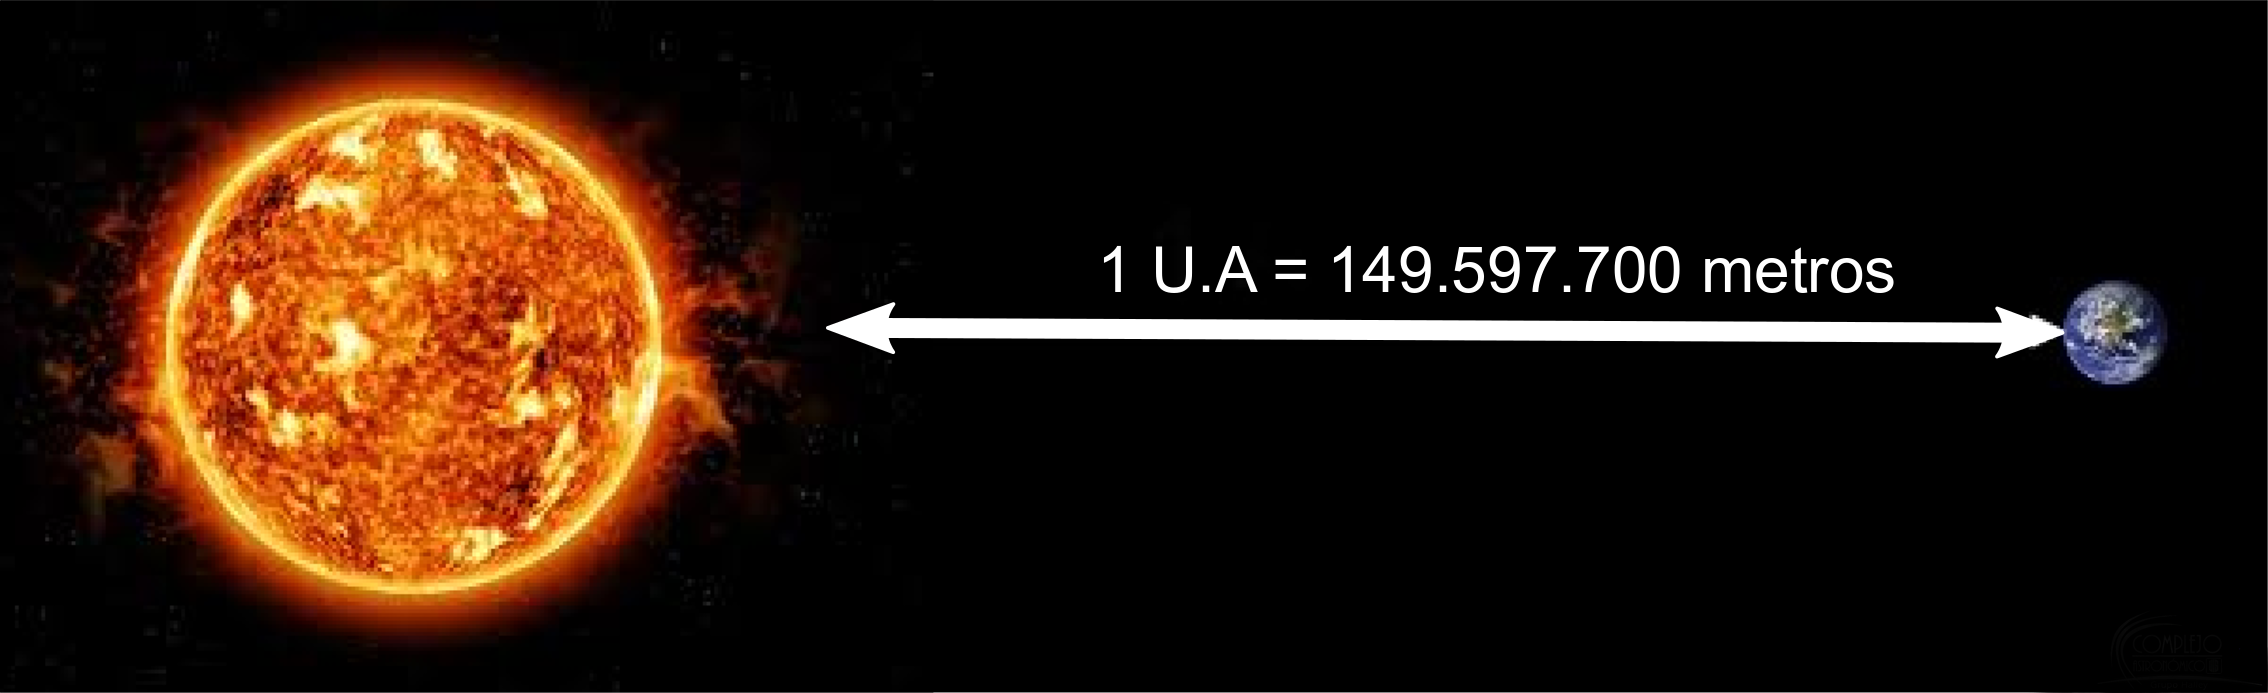
\includegraphics[scale=0.2]{Imagenes/Unidad_astro_01}
  \end{figure}
\end{frame}

\begin{frame}{Distancias y tamaños en el Sistema Solar}
  \begin{figure}
   \centering
   %\raggedright
   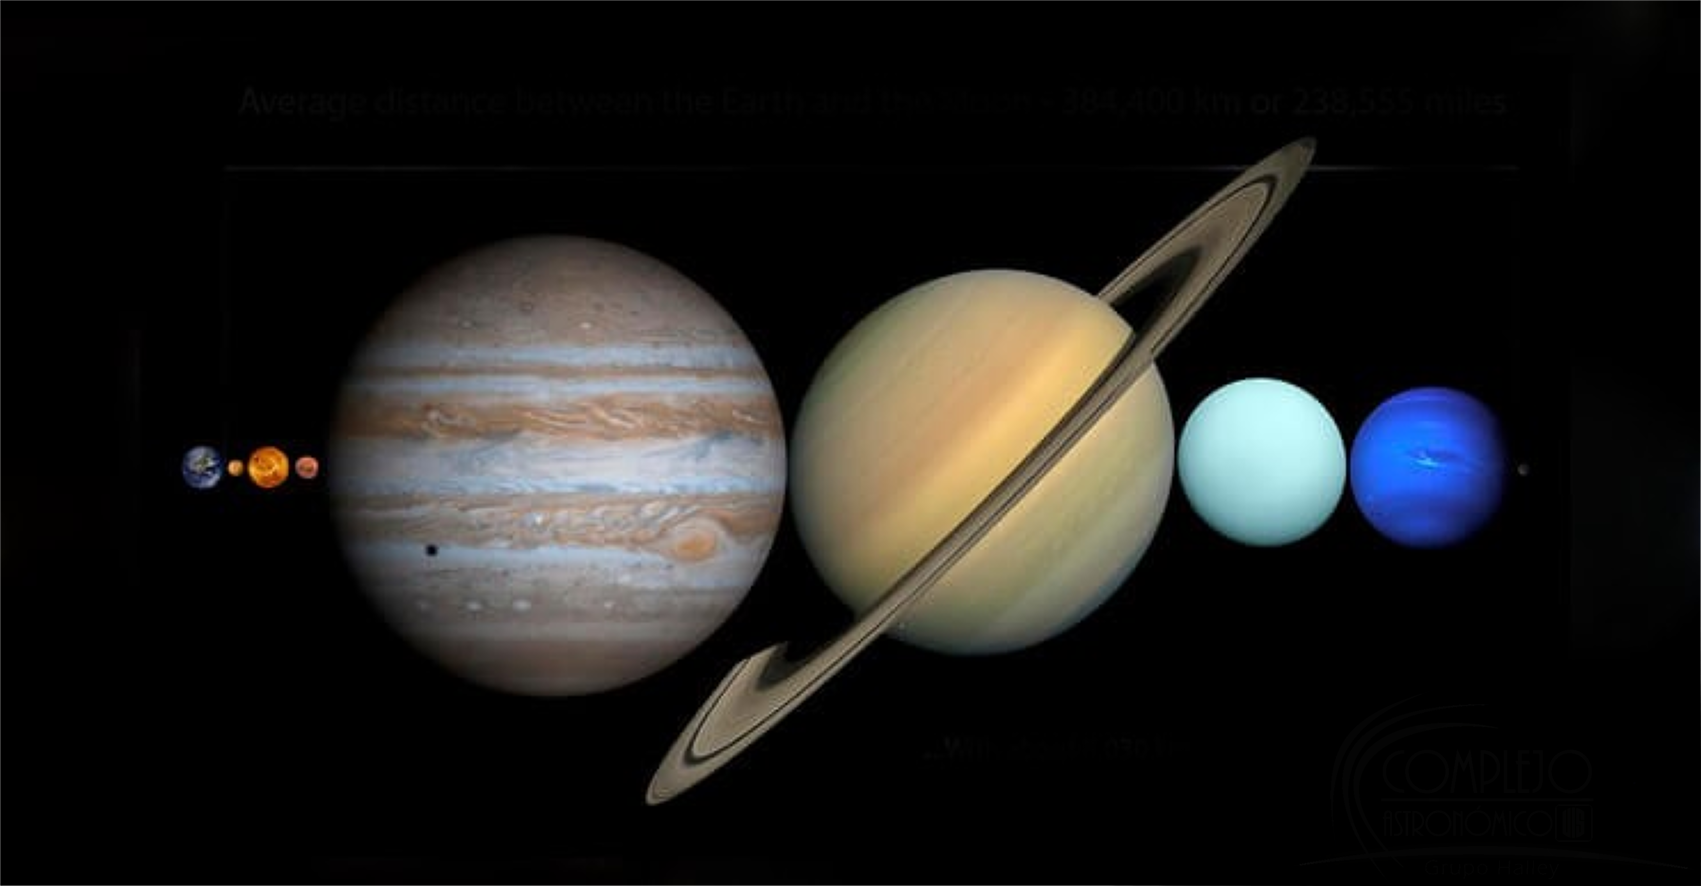
\includegraphics[scale=0.23]{Imagenes/Tamanos_01}
  \end{figure}
\end{frame}

\begin{frame}{Distancias}
\begin{table}[H]
\begin{tabular}{|c|c|c|}
\hline
\textbf{Objeto}   & \textbf{Distancia al Sol{[}km{]}}                                      & \textbf{Distancia al Sol  {[}cm{]}} \\ \hline
\textbf{Mercurio} &  57.910.000    & 5.791                   \\ \hline
\textbf{Venus}    & 108.200.000   & 10.82                   \\ \hline
\textbf{Tierra}   & 146.600.000  & 14.66                   \\ \hline
\textbf{Marte}    & 227.940.000    & 22.794                  \\ \hline
\textbf{Júpiter}  & 778.330.000   & 77.833                  \\ \hline
\textbf{Saturno}  & 1.429.400.000 & 142.94                  \\ \hline
\textbf{Urano}    & 2.870.990.000   & 287.099                 \\ \hline
\textbf{Neptuno}  & 4.504.300.000     & 450.43                  \\ \hline
\end{tabular}
\end{table}
\end{frame}

\begin{frame}{Tamaños}
\begin{table}[H]
\begin{tabular}{|c|c|c|}
\hline
\textbf{Objeto}   & \textbf{Radio {[}km{]}}                               & \textbf{Radio {[}cm{]}} \\ \hline
\textbf{Sol}      & 696.340                                               & 139.268                 \\ \hline
\textbf{Mercurio} &  2.44  & 0.48                    \\ \hline
\textbf{Venus}    & 6.052  & 1.21           \\ \hline
\textbf{Tierra}   & 6.378                                                 & 1.28                    \\ \hline
\textbf{Marte}    & 3.397   & 0.68                    \\ \hline
\textbf{Júpiter}  &  71.492 & 14.30            \\ \hline
\textbf{Saturno}  &60.268 & 12.05       \\ \hline
\textbf{Urano}    & 25.559                                                & 5.11                    \\ \hline
\textbf{Neptuno}  & 24.746                                                & 4.94                    \\ \hline
\end{tabular}
\end{table}
\end{frame}

\begin{frame}{Paralaje}
  \begin{figure}
   \centering
   %\raggedright
   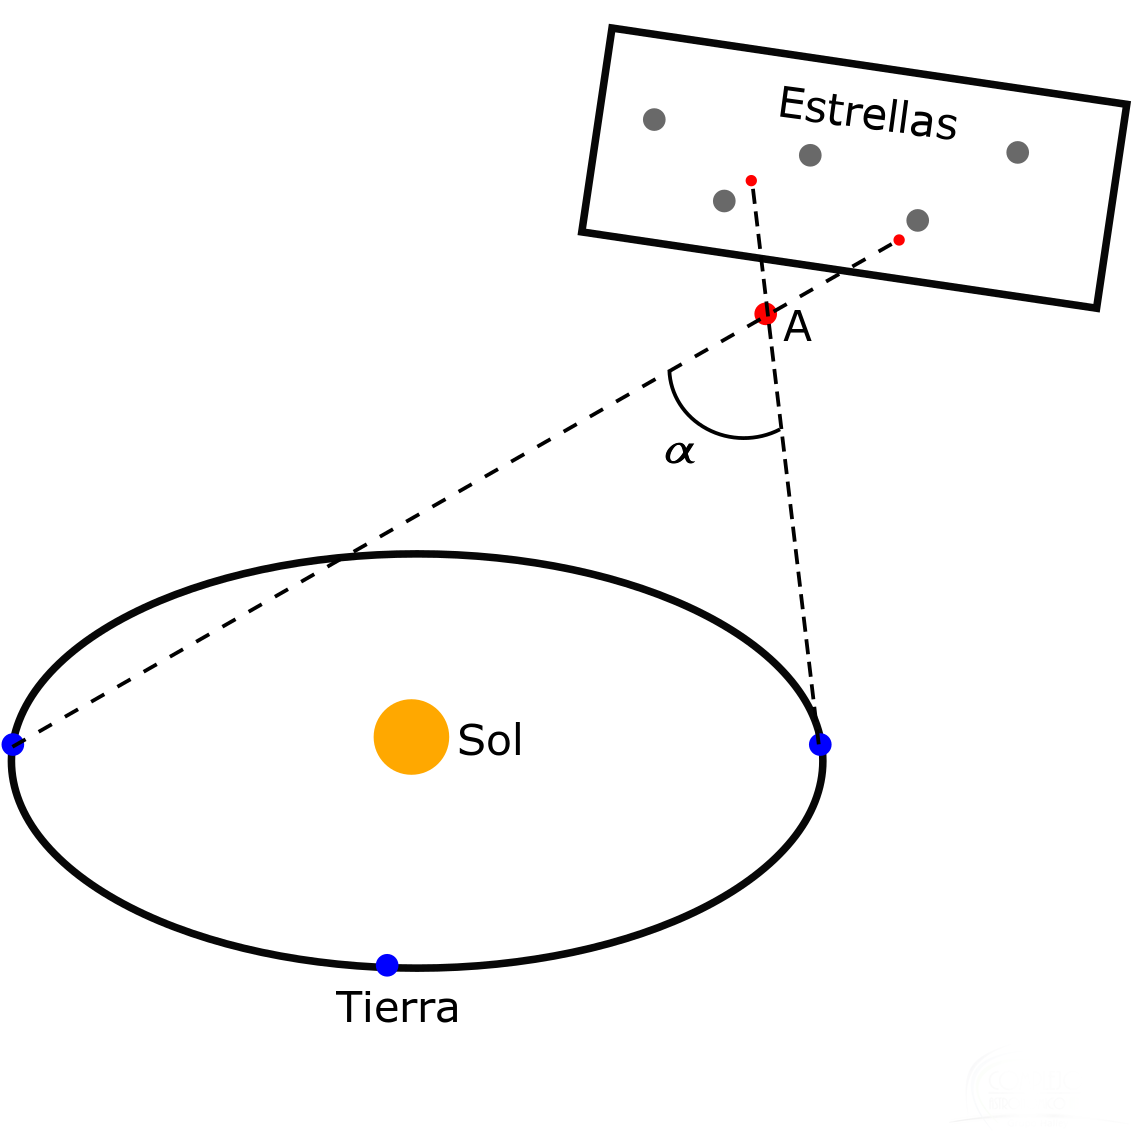
\includegraphics[scale=0.23]{Imagenes/Paralaje_01}
  \end{figure}
\end{frame}

\begin{frame}{Paralaje - ejercicio 1}
  \begin{figure}
   \centering
   %\raggedright
   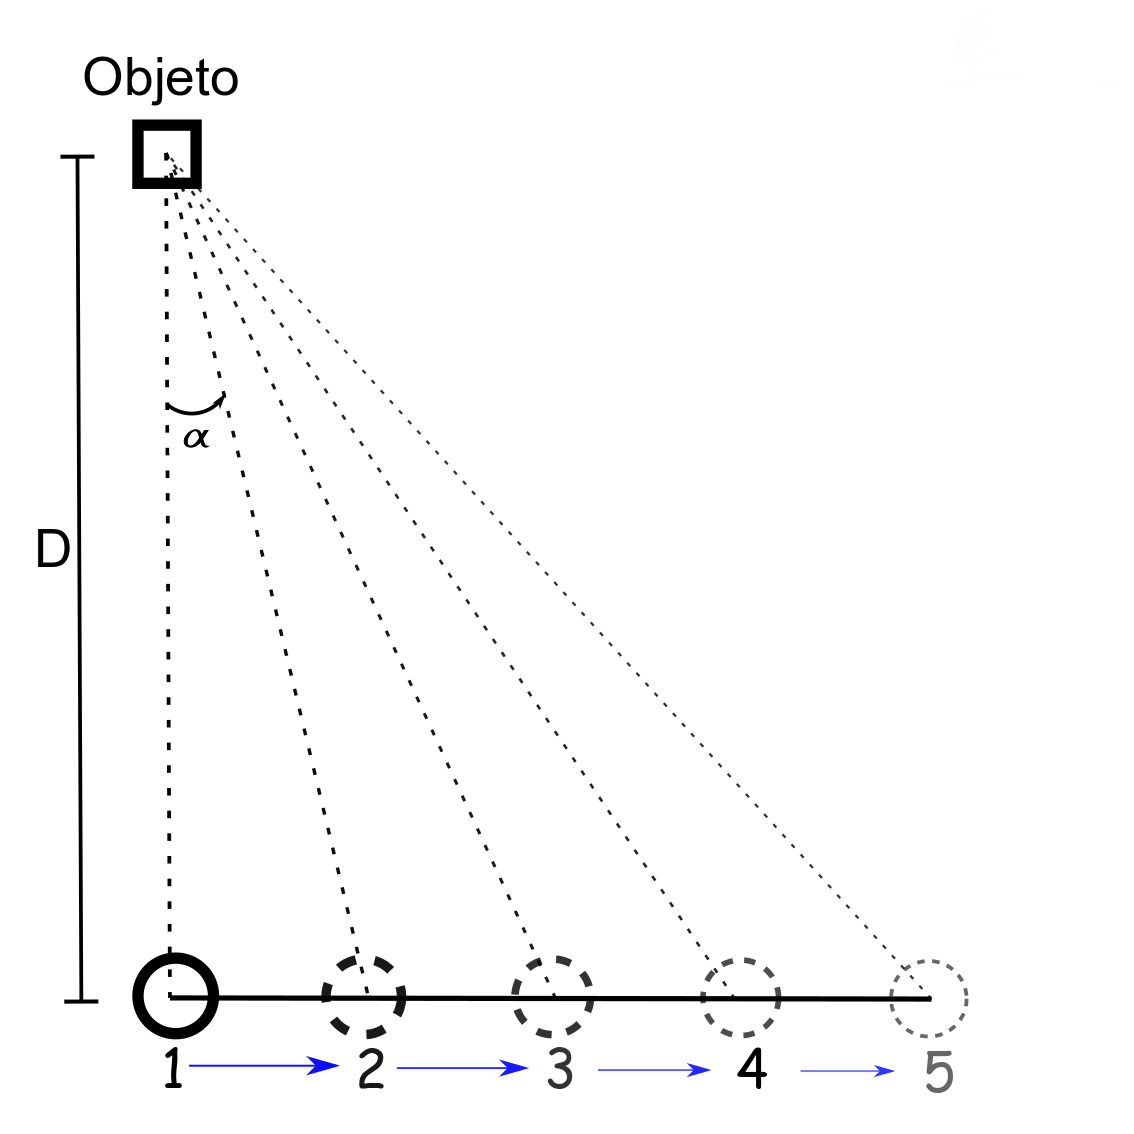
\includegraphics[scale=0.23]{Imagenes/Paralaje_02}
  \end{figure}
\end{frame}


\begin{frame}{Paralaje - ejercicio 2}
  \begin{figure}
   \centering
   %\raggedright
   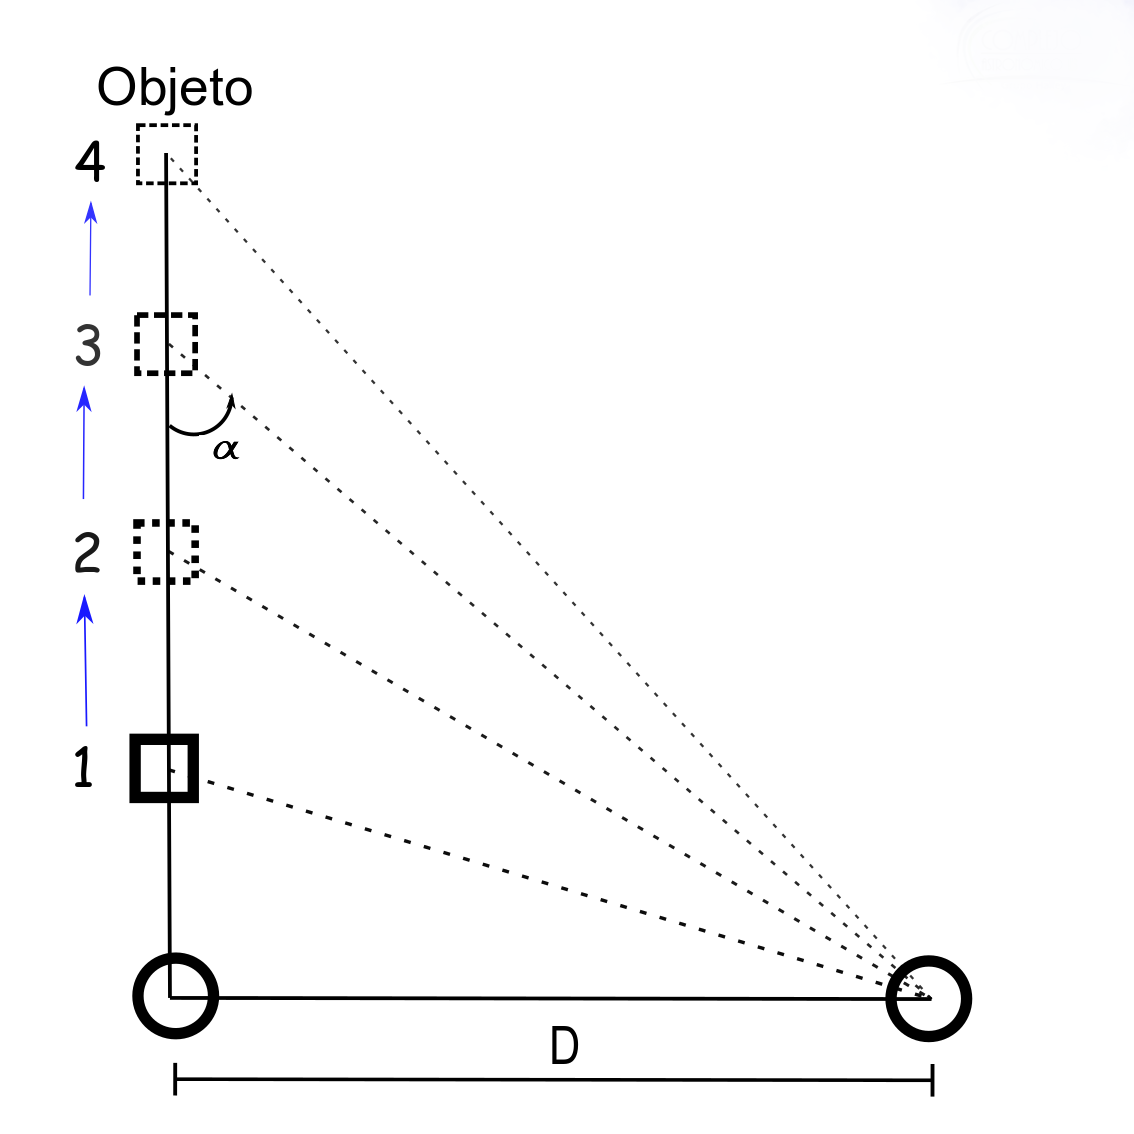
\includegraphics[scale=0.23]{Imagenes/Paralaje_03}
  \end{figure}
\end{frame}

\begin{frame}
\begin{center}
\Huge 
\textit{``Dos cosas son infinitas: la estupidez humana y el universo; y no estoy seguro de lo segundo"}
\end{center}
\begin{flushright}
\small
\textit{Albert Einstein}
\end{flushright}
\end{frame}

\end{document}